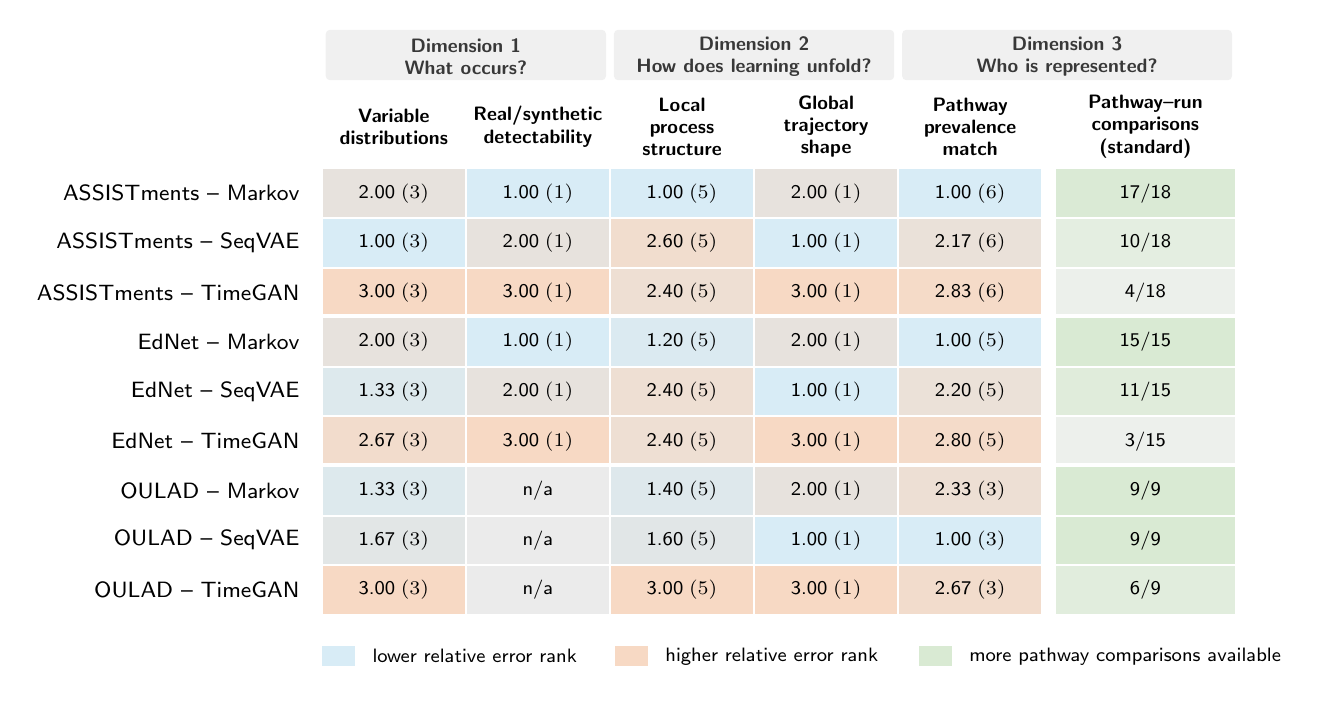
\begin{tikzpicture}[x=1cm,y=1cm,font=\sffamily]
\definecolor{rankbest}{HTML}{D8ECF6}
\definecolor{rankworst}{HTML}{F7D9C4}
\definecolor{supportbest}{HTML}{D9EAD3}
\definecolor{supportworst}{HTML}{F2F2F2}
\fill[black!6,rounded corners=1.5pt] (4.050,1.760) rectangle (7.610,1.120);
\node[align=center,font=\sffamily\bfseries\scriptsize,text=black!78] at (5.830,1.420) {Dimension 1\\What occurs?};
\fill[black!6,rounded corners=1.5pt] (7.710,1.760) rectangle (11.270,1.120);
\node[align=center,font=\sffamily\bfseries\scriptsize,text=black!78] at (9.490,1.420) {Dimension 2\\How does learning unfold?};
\fill[black!6,rounded corners=1.5pt] (11.370,1.760) rectangle (15.560,1.120);
\node[align=center,font=\sffamily\bfseries\scriptsize,text=black!78] at (13.465,1.420) {Dimension 3\\Who is represented?};
\node[align=center,font=\sffamily\bfseries\scriptsize] at (4.915,0.530) {Variable\\distributions};
\node[align=center,font=\sffamily\bfseries\scriptsize] at (6.745,0.530) {Real/synthetic\\detectability};
\node[align=center,font=\sffamily\bfseries\scriptsize] at (8.575,0.530) {Local\\process\\structure};
\node[align=center,font=\sffamily\bfseries\scriptsize] at (10.405,0.530) {Global\\trajectory\\shape};
\node[align=center,font=\sffamily\bfseries\scriptsize] at (12.235,0.530) {Pathway\\prevalence\\match};
\node[align=center,font=\sffamily\bfseries\scriptsize] at (14.460,0.530) {Pathway--run\\comparisons\\(standard)};
\node[anchor=east,font=\sffamily\footnotesize] at (3.840,-0.315) {ASSISTments -- Markov};
\fill[rankbest!50!rankworst] (4.000,0.000) rectangle (5.830,-0.630);
\draw[white,line width=0.7pt] (4.000,0.000) rectangle (5.830,-0.630);
\node[align=center,font=\sffamily\scriptsize] at (4.915,-0.315) {2.00\;\textnormal{(3)}};
\fill[rankbest!100!rankworst] (5.830,0.000) rectangle (7.660,-0.630);
\draw[white,line width=0.7pt] (5.830,0.000) rectangle (7.660,-0.630);
\node[align=center,font=\sffamily\scriptsize] at (6.745,-0.315) {1.00\;\textnormal{(1)}};
\fill[rankbest!100!rankworst] (7.660,0.000) rectangle (9.490,-0.630);
\draw[white,line width=0.7pt] (7.660,0.000) rectangle (9.490,-0.630);
\node[align=center,font=\sffamily\scriptsize] at (8.575,-0.315) {1.00\;\textnormal{(5)}};
\fill[rankbest!50!rankworst] (9.490,0.000) rectangle (11.320,-0.630);
\draw[white,line width=0.7pt] (9.490,0.000) rectangle (11.320,-0.630);
\node[align=center,font=\sffamily\scriptsize] at (10.405,-0.315) {2.00\;\textnormal{(1)}};
\fill[rankbest!100!rankworst] (11.320,0.000) rectangle (13.150,-0.630);
\draw[white,line width=0.7pt] (11.320,0.000) rectangle (13.150,-0.630);
\node[align=center,font=\sffamily\scriptsize] at (12.235,-0.315) {1.00\;\textnormal{(6)}};
\fill[supportbest!94!supportworst] (13.310,0.000) rectangle (15.610,-0.630);
\draw[white,line width=0.7pt] (13.310,0.000) rectangle (15.610,-0.630);
\node[align=center,font=\sffamily\scriptsize] at (14.460,-0.315) {17/18};
\node[anchor=east,font=\sffamily\footnotesize] at (3.840,-0.945) {ASSISTments -- SeqVAE};
\fill[rankbest!100!rankworst] (4.000,-0.630) rectangle (5.830,-1.260);
\draw[white,line width=0.7pt] (4.000,-0.630) rectangle (5.830,-1.260);
\node[align=center,font=\sffamily\scriptsize] at (4.915,-0.945) {1.00\;\textnormal{(3)}};
\fill[rankbest!50!rankworst] (5.830,-0.630) rectangle (7.660,-1.260);
\draw[white,line width=0.7pt] (5.830,-0.630) rectangle (7.660,-1.260);
\node[align=center,font=\sffamily\scriptsize] at (6.745,-0.945) {2.00\;\textnormal{(1)}};
\fill[rankbest!20!rankworst] (7.660,-0.630) rectangle (9.490,-1.260);
\draw[white,line width=0.7pt] (7.660,-0.630) rectangle (9.490,-1.260);
\node[align=center,font=\sffamily\scriptsize] at (8.575,-0.945) {2.60\;\textnormal{(5)}};
\fill[rankbest!100!rankworst] (9.490,-0.630) rectangle (11.320,-1.260);
\draw[white,line width=0.7pt] (9.490,-0.630) rectangle (11.320,-1.260);
\node[align=center,font=\sffamily\scriptsize] at (10.405,-0.945) {1.00\;\textnormal{(1)}};
\fill[rankbest!42!rankworst] (11.320,-0.630) rectangle (13.150,-1.260);
\draw[white,line width=0.7pt] (11.320,-0.630) rectangle (13.150,-1.260);
\node[align=center,font=\sffamily\scriptsize] at (12.235,-0.945) {2.17\;\textnormal{(6)}};
\fill[supportbest!56!supportworst] (13.310,-0.630) rectangle (15.610,-1.260);
\draw[white,line width=0.7pt] (13.310,-0.630) rectangle (15.610,-1.260);
\node[align=center,font=\sffamily\scriptsize] at (14.460,-0.945) {10/18};
\node[anchor=east,font=\sffamily\footnotesize] at (3.840,-1.575) {ASSISTments -- TimeGAN};
\fill[rankbest!0!rankworst] (4.000,-1.260) rectangle (5.830,-1.890);
\draw[white,line width=0.7pt] (4.000,-1.260) rectangle (5.830,-1.890);
\node[align=center,font=\sffamily\scriptsize] at (4.915,-1.575) {3.00\;\textnormal{(3)}};
\fill[rankbest!0!rankworst] (5.830,-1.260) rectangle (7.660,-1.890);
\draw[white,line width=0.7pt] (5.830,-1.260) rectangle (7.660,-1.890);
\node[align=center,font=\sffamily\scriptsize] at (6.745,-1.575) {3.00\;\textnormal{(1)}};
\fill[rankbest!30!rankworst] (7.660,-1.260) rectangle (9.490,-1.890);
\draw[white,line width=0.7pt] (7.660,-1.260) rectangle (9.490,-1.890);
\node[align=center,font=\sffamily\scriptsize] at (8.575,-1.575) {2.40\;\textnormal{(5)}};
\fill[rankbest!0!rankworst] (9.490,-1.260) rectangle (11.320,-1.890);
\draw[white,line width=0.7pt] (9.490,-1.260) rectangle (11.320,-1.890);
\node[align=center,font=\sffamily\scriptsize] at (10.405,-1.575) {3.00\;\textnormal{(1)}};
\fill[rankbest!8!rankworst] (11.320,-1.260) rectangle (13.150,-1.890);
\draw[white,line width=0.7pt] (11.320,-1.260) rectangle (13.150,-1.890);
\node[align=center,font=\sffamily\scriptsize] at (12.235,-1.575) {2.83\;\textnormal{(6)}};
\fill[supportbest!22!supportworst] (13.310,-1.260) rectangle (15.610,-1.890);
\draw[white,line width=0.7pt] (13.310,-1.260) rectangle (15.610,-1.890);
\node[align=center,font=\sffamily\scriptsize] at (14.460,-1.575) {4/18};
\draw[white,line width=2.2pt] (4.000,-1.890) -- (15.610,-1.890);
\node[anchor=east,font=\sffamily\footnotesize] at (3.840,-2.205) {EdNet -- Markov};
\fill[rankbest!50!rankworst] (4.000,-1.890) rectangle (5.830,-2.520);
\draw[white,line width=0.7pt] (4.000,-1.890) rectangle (5.830,-2.520);
\node[align=center,font=\sffamily\scriptsize] at (4.915,-2.205) {2.00\;\textnormal{(3)}};
\fill[rankbest!100!rankworst] (5.830,-1.890) rectangle (7.660,-2.520);
\draw[white,line width=0.7pt] (5.830,-1.890) rectangle (7.660,-2.520);
\node[align=center,font=\sffamily\scriptsize] at (6.745,-2.205) {1.00\;\textnormal{(1)}};
\fill[rankbest!90!rankworst] (7.660,-1.890) rectangle (9.490,-2.520);
\draw[white,line width=0.7pt] (7.660,-1.890) rectangle (9.490,-2.520);
\node[align=center,font=\sffamily\scriptsize] at (8.575,-2.205) {1.20\;\textnormal{(5)}};
\fill[rankbest!50!rankworst] (9.490,-1.890) rectangle (11.320,-2.520);
\draw[white,line width=0.7pt] (9.490,-1.890) rectangle (11.320,-2.520);
\node[align=center,font=\sffamily\scriptsize] at (10.405,-2.205) {2.00\;\textnormal{(1)}};
\fill[rankbest!100!rankworst] (11.320,-1.890) rectangle (13.150,-2.520);
\draw[white,line width=0.7pt] (11.320,-1.890) rectangle (13.150,-2.520);
\node[align=center,font=\sffamily\scriptsize] at (12.235,-2.205) {1.00\;\textnormal{(5)}};
\fill[supportbest!100!supportworst] (13.310,-1.890) rectangle (15.610,-2.520);
\draw[white,line width=0.7pt] (13.310,-1.890) rectangle (15.610,-2.520);
\node[align=center,font=\sffamily\scriptsize] at (14.460,-2.205) {15/15};
\node[anchor=east,font=\sffamily\footnotesize] at (3.840,-2.835) {EdNet -- SeqVAE};
\fill[rankbest!83!rankworst] (4.000,-2.520) rectangle (5.830,-3.150);
\draw[white,line width=0.7pt] (4.000,-2.520) rectangle (5.830,-3.150);
\node[align=center,font=\sffamily\scriptsize] at (4.915,-2.835) {1.33\;\textnormal{(3)}};
\fill[rankbest!50!rankworst] (5.830,-2.520) rectangle (7.660,-3.150);
\draw[white,line width=0.7pt] (5.830,-2.520) rectangle (7.660,-3.150);
\node[align=center,font=\sffamily\scriptsize] at (6.745,-2.835) {2.00\;\textnormal{(1)}};
\fill[rankbest!30!rankworst] (7.660,-2.520) rectangle (9.490,-3.150);
\draw[white,line width=0.7pt] (7.660,-2.520) rectangle (9.490,-3.150);
\node[align=center,font=\sffamily\scriptsize] at (8.575,-2.835) {2.40\;\textnormal{(5)}};
\fill[rankbest!100!rankworst] (9.490,-2.520) rectangle (11.320,-3.150);
\draw[white,line width=0.7pt] (9.490,-2.520) rectangle (11.320,-3.150);
\node[align=center,font=\sffamily\scriptsize] at (10.405,-2.835) {1.00\;\textnormal{(1)}};
\fill[rankbest!40!rankworst] (11.320,-2.520) rectangle (13.150,-3.150);
\draw[white,line width=0.7pt] (11.320,-2.520) rectangle (13.150,-3.150);
\node[align=center,font=\sffamily\scriptsize] at (12.235,-2.835) {2.20\;\textnormal{(5)}};
\fill[supportbest!73!supportworst] (13.310,-2.520) rectangle (15.610,-3.150);
\draw[white,line width=0.7pt] (13.310,-2.520) rectangle (15.610,-3.150);
\node[align=center,font=\sffamily\scriptsize] at (14.460,-2.835) {11/15};
\node[anchor=east,font=\sffamily\footnotesize] at (3.840,-3.465) {EdNet -- TimeGAN};
\fill[rankbest!17!rankworst] (4.000,-3.150) rectangle (5.830,-3.780);
\draw[white,line width=0.7pt] (4.000,-3.150) rectangle (5.830,-3.780);
\node[align=center,font=\sffamily\scriptsize] at (4.915,-3.465) {2.67\;\textnormal{(3)}};
\fill[rankbest!0!rankworst] (5.830,-3.150) rectangle (7.660,-3.780);
\draw[white,line width=0.7pt] (5.830,-3.150) rectangle (7.660,-3.780);
\node[align=center,font=\sffamily\scriptsize] at (6.745,-3.465) {3.00\;\textnormal{(1)}};
\fill[rankbest!30!rankworst] (7.660,-3.150) rectangle (9.490,-3.780);
\draw[white,line width=0.7pt] (7.660,-3.150) rectangle (9.490,-3.780);
\node[align=center,font=\sffamily\scriptsize] at (8.575,-3.465) {2.40\;\textnormal{(5)}};
\fill[rankbest!0!rankworst] (9.490,-3.150) rectangle (11.320,-3.780);
\draw[white,line width=0.7pt] (9.490,-3.150) rectangle (11.320,-3.780);
\node[align=center,font=\sffamily\scriptsize] at (10.405,-3.465) {3.00\;\textnormal{(1)}};
\fill[rankbest!10!rankworst] (11.320,-3.150) rectangle (13.150,-3.780);
\draw[white,line width=0.7pt] (11.320,-3.150) rectangle (13.150,-3.780);
\node[align=center,font=\sffamily\scriptsize] at (12.235,-3.465) {2.80\;\textnormal{(5)}};
\fill[supportbest!20!supportworst] (13.310,-3.150) rectangle (15.610,-3.780);
\draw[white,line width=0.7pt] (13.310,-3.150) rectangle (15.610,-3.780);
\node[align=center,font=\sffamily\scriptsize] at (14.460,-3.465) {3/15};
\draw[white,line width=2.2pt] (4.000,-3.780) -- (15.610,-3.780);
\node[anchor=east,font=\sffamily\footnotesize] at (3.840,-4.095) {OULAD -- Markov};
\fill[rankbest!83!rankworst] (4.000,-3.780) rectangle (5.830,-4.410);
\draw[white,line width=0.7pt] (4.000,-3.780) rectangle (5.830,-4.410);
\node[align=center,font=\sffamily\scriptsize] at (4.915,-4.095) {1.33\;\textnormal{(3)}};
\fill[gray!16] (5.830,-3.780) rectangle (7.660,-4.410);
\draw[white,line width=0.7pt] (5.830,-3.780) rectangle (7.660,-4.410);
\node[align=center,font=\sffamily\scriptsize] at (6.745,-4.095) {n/a};
\fill[rankbest!80!rankworst] (7.660,-3.780) rectangle (9.490,-4.410);
\draw[white,line width=0.7pt] (7.660,-3.780) rectangle (9.490,-4.410);
\node[align=center,font=\sffamily\scriptsize] at (8.575,-4.095) {1.40\;\textnormal{(5)}};
\fill[rankbest!50!rankworst] (9.490,-3.780) rectangle (11.320,-4.410);
\draw[white,line width=0.7pt] (9.490,-3.780) rectangle (11.320,-4.410);
\node[align=center,font=\sffamily\scriptsize] at (10.405,-4.095) {2.00\;\textnormal{(1)}};
\fill[rankbest!33!rankworst] (11.320,-3.780) rectangle (13.150,-4.410);
\draw[white,line width=0.7pt] (11.320,-3.780) rectangle (13.150,-4.410);
\node[align=center,font=\sffamily\scriptsize] at (12.235,-4.095) {2.33\;\textnormal{(3)}};
\fill[supportbest!100!supportworst] (13.310,-3.780) rectangle (15.610,-4.410);
\draw[white,line width=0.7pt] (13.310,-3.780) rectangle (15.610,-4.410);
\node[align=center,font=\sffamily\scriptsize] at (14.460,-4.095) {9/9};
\node[anchor=east,font=\sffamily\footnotesize] at (3.840,-4.725) {OULAD -- SeqVAE};
\fill[rankbest!67!rankworst] (4.000,-4.410) rectangle (5.830,-5.040);
\draw[white,line width=0.7pt] (4.000,-4.410) rectangle (5.830,-5.040);
\node[align=center,font=\sffamily\scriptsize] at (4.915,-4.725) {1.67\;\textnormal{(3)}};
\fill[gray!16] (5.830,-4.410) rectangle (7.660,-5.040);
\draw[white,line width=0.7pt] (5.830,-4.410) rectangle (7.660,-5.040);
\node[align=center,font=\sffamily\scriptsize] at (6.745,-4.725) {n/a};
\fill[rankbest!70!rankworst] (7.660,-4.410) rectangle (9.490,-5.040);
\draw[white,line width=0.7pt] (7.660,-4.410) rectangle (9.490,-5.040);
\node[align=center,font=\sffamily\scriptsize] at (8.575,-4.725) {1.60\;\textnormal{(5)}};
\fill[rankbest!100!rankworst] (9.490,-4.410) rectangle (11.320,-5.040);
\draw[white,line width=0.7pt] (9.490,-4.410) rectangle (11.320,-5.040);
\node[align=center,font=\sffamily\scriptsize] at (10.405,-4.725) {1.00\;\textnormal{(1)}};
\fill[rankbest!100!rankworst] (11.320,-4.410) rectangle (13.150,-5.040);
\draw[white,line width=0.7pt] (11.320,-4.410) rectangle (13.150,-5.040);
\node[align=center,font=\sffamily\scriptsize] at (12.235,-4.725) {1.00\;\textnormal{(3)}};
\fill[supportbest!100!supportworst] (13.310,-4.410) rectangle (15.610,-5.040);
\draw[white,line width=0.7pt] (13.310,-4.410) rectangle (15.610,-5.040);
\node[align=center,font=\sffamily\scriptsize] at (14.460,-4.725) {9/9};
\node[anchor=east,font=\sffamily\footnotesize] at (3.840,-5.355) {OULAD -- TimeGAN};
\fill[rankbest!0!rankworst] (4.000,-5.040) rectangle (5.830,-5.670);
\draw[white,line width=0.7pt] (4.000,-5.040) rectangle (5.830,-5.670);
\node[align=center,font=\sffamily\scriptsize] at (4.915,-5.355) {3.00\;\textnormal{(3)}};
\fill[gray!16] (5.830,-5.040) rectangle (7.660,-5.670);
\draw[white,line width=0.7pt] (5.830,-5.040) rectangle (7.660,-5.670);
\node[align=center,font=\sffamily\scriptsize] at (6.745,-5.355) {n/a};
\fill[rankbest!0!rankworst] (7.660,-5.040) rectangle (9.490,-5.670);
\draw[white,line width=0.7pt] (7.660,-5.040) rectangle (9.490,-5.670);
\node[align=center,font=\sffamily\scriptsize] at (8.575,-5.355) {3.00\;\textnormal{(5)}};
\fill[rankbest!0!rankworst] (9.490,-5.040) rectangle (11.320,-5.670);
\draw[white,line width=0.7pt] (9.490,-5.040) rectangle (11.320,-5.670);
\node[align=center,font=\sffamily\scriptsize] at (10.405,-5.355) {3.00\;\textnormal{(1)}};
\fill[rankbest!17!rankworst] (11.320,-5.040) rectangle (13.150,-5.670);
\draw[white,line width=0.7pt] (11.320,-5.040) rectangle (13.150,-5.670);
\node[align=center,font=\sffamily\scriptsize] at (12.235,-5.355) {2.67\;\textnormal{(3)}};
\fill[supportbest!67!supportworst] (13.310,-5.040) rectangle (15.610,-5.670);
\draw[white,line width=0.7pt] (13.310,-5.040) rectangle (15.610,-5.670);
\node[align=center,font=\sffamily\scriptsize] at (14.460,-5.355) {6/9};
\fill[rankbest] (4.000,-6.070) rectangle (4.420,-6.320);
\node[anchor=west,font=\sffamily\scriptsize] at (4.520,-6.195) {lower relative error rank};
\fill[rankworst] (7.720,-6.070) rectangle (8.140,-6.320);
\node[anchor=west,font=\sffamily\scriptsize] at (8.240,-6.195) {higher relative error rank};
\fill[supportbest] (11.580,-6.070) rectangle (12.000,-6.320);
\node[anchor=west,font=\sffamily\scriptsize] at (12.100,-6.195) {more pathway comparisons available};
\end{tikzpicture}
